\documentclass[titlepage]{article}
\usepackage[bottom=3cm, right=2cm, left=2cm, top=3cm]{geometry}
\usepackage{graphicx}
\usepackage{hyperref}
\usepackage{float}
\restylefloat{table}
\usepackage{amsmath}
\usepackage{booktabs}

\title{SFWRENG 4NL3 Assignment 4: \\ Pretrained Transformers}
\author{Sumanya Gulati}
\date{1 April 2025}

\begin{document}

\begin{titlepage}
    \maketitle
\end{titlepage}

\newpage 

\tableofcontents
\listoftables
\listoffigures

\newpage

\section{Dataset}
For this assignment, I am using the GoEmotions dataset extracted from the HuggingFace can be accessed 
\href{https://huggingface.co/datasets/google-research-datasets/go_emotions}{here}. The task at hand 
involves emotion classification, aiming to identify and categorize the emotions expressed in textual data. This 
is essential for applications such as sentiment analysis, mental health assessment, enhancing human-computer 
interactions and more. \\

The GoEmotions dataset comprises of about 58,000 English Reddit comments, each annotated for 27 distinct emotion 
categories or marked as neutral. The simplified version of the dataset with predefined train, val and test splits 
has been used for this assignment. 

\subsection{Data Collection}
The dataset has been constructed by selecting English-language comments from Reddit by researchers at Amazon Alexa, 
Google Research and Stanford Linguistics. A complete list of authors can be found \href{https://arxiv.org/abs/2005.00547}
{here}. The comments were extracted from Reddit using a variety of automated methods along with data curation techniques 
such as reducing profanity, length filtering, sentiment and emotion balancing, masking and more. Further information 
about the data collection process can be found in section 3.1 of \href{https://arxiv.org/pdf/2005.00547}{this paper}.

\subsection{Dataset Structure}
Each instance of the dataset corresponds to a reddit comment with an ID and one or more emotion annotations including neutral.
The simplified configuration of the dataset which has been used for this assignment, includes:

\begin{itemize}
    \item \texttt{text}: the Reddit comment
    \item \texttt{labels}: the emotional annotations
    \item \texttt{comment\_id}: a unique identifier for the comment
\end{itemize}

The input for the task is a Reddit comment in English and the corresponding output is a set of one or more labels corresponding 
to the 27 emotion categories or neutral, reflecting the emotional content of the comment.

The labels are stored as a list of integers ranging from 0 to 27 where each integer represents an emotion category or neutral. The 
label mapping is as follows:

\begin{table}[H] \label{tab:labels}
    \centering
    \begin{tabular}{lll}
    \toprule
    \textbf{Label Number} & \textbf{Label Category} \\
    \midrule
    0 & admiration \\
    1 & amusement \\
    2 & anger \\
    3 & annoyance \\
    4 & approval \\
    5 & caring \\ 
    6 & confusion \\
    7 & curiosity \\
    8 & desire \\
    9 & disappointment \\
    10 & disapproval \\
    11 & disgust \\
    12 & embarrassment \\
    13 & excitement \\
    14 & fear \\
    15 & gratitude \\
    16 & grief \\
    17 & joy \\
    18 & love \\
    19 & nervousness \\
    20 & optimism \\
    21 & pride \\
    22 & realization \\
    23 & relief \\
    24 & remorse \\
    25 & sadness \\
    26 & surprise \\
    27 & neutral \\
    \bottomrule
    \end{tabular}
    \caption{Label Mapping}
\end{table}

\subsection{Evaluation Metrics}
The following evaluation metrics have been used to assess the performance of the BERT-based model:
\begin{itemize}
    \item Model Performance:
        \begin{itemize}
            \item Emotion-level Precision, Recall, F1: Measured per each emotion in the GoEmotions taxonomy.
            \item Transfer Learning: F1 score on data transferred between domain X and GoEmotions.
        \end{itemize}
    \item Decision thresholds: No thresholds are used. The data is presented in full granularity.
    \item Uncertainty and variability: Repeated experiments have yielded results with similar taxonomical rankings.
\end{itemize}

The model has been evaluated on 10 publicly available datasets including 9 benchmark datasets presented in compilation 
by \href{https://aclanthology.org/C18-1179/}{Bostan and Klinger} and the \href{https://github.com/google-research/google-research/tree/master/goemotions}
{GoEmotions} eval set. Full details about the evaludation results can be found in the \href{https://arxiv.org/pdf/2005.00547}{paper}.

To summarize, based on the information derived from the dataset, the following evaluation metrics will be used for this assignment:
\begin{enumerate}
    \item \textbf{Loss}: The loss value on the evaluation dataset. 
    \item \textbf{F1 Score}: The model's accuracy on a scale of 0 to 1 with 1 being perfect accuracy.
    \item \textbf{Runtime}: Time taken to complete the evaluation.
    \item \textbf{Samples per Second}: The processing speed of the model, as in, how many data samples are evaluated by the model per second.
    \item \textbf{Steps per Second}: How many evaluation steps or batches were processed per second.
    \item \textbf{Epoch}: A measure of how far the training process of the evaluation was taken. One epoch refers to one complete 
    pass through the training dataset.
\end{enumerate}

\subsection{Data Splits}
The dataset is divided into training, validating and test splits as follows:

\begin{table}[H] \label{tab:data_split}
    \centering
    \begin{tabular}{lll}
    \toprule
    \textbf{Data Split} & \textbf{Number of Instances} \\
    \midrule
    Training & 43,410 \\
    Validation & 5,426 \\
    Test & 5,427 \\
    \bottomrule
    \end{tabular}
    \caption{Data Split Overview}
\end{table}

Class distributions for the training and test splits are shown in the figure \ref{fig:class_distribution}.

\begin{figure}[H] \label{fig:class_distribution}
    \centering
    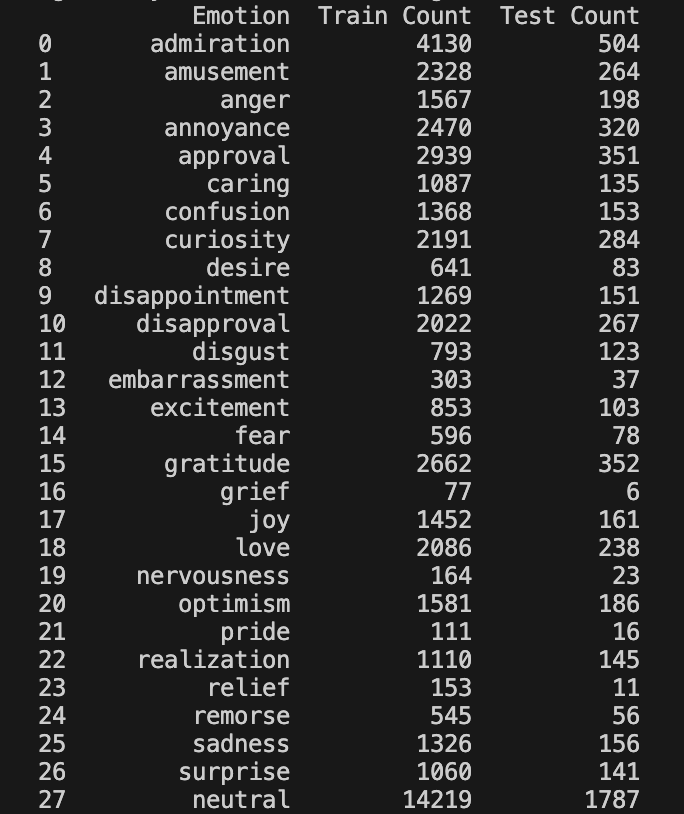
\includegraphics[scale=0.8]{/Users/sg/Desktop/courses/winter-2025/4nl3/assignments/assignment-4/homework4_report/figures/class_distributions.png}
    \caption{Class Distribution in Training and Test Splits}
\end{figure}

\subsection{Additional Features}
Although the comments vary in length, the maximum sequence length has been capped at 30 tokens in the training and evaludation datasets 
to ensure concise and focused emotional expressions. Furthermore, linguistic context consistency has been ensured by only choosing comments 
that are in English.
 
\section{Fine-tuned Models}
For this task, the \href{https://huggingface.co/FacebookAI/roberta-base}{RoBERTa-base} model and the \href{https://huggingface.co/distilbert/distilbert-base-uncased}
{DistilBERT-base-uncased} model have been used. 

\subsection{Model 1: RoBERTa-base}
RoBERTa or "A Robustly Optimized BERT Pretraining Approach" is a transformer-based model that builds on the BERT architecture. It improves upon 
BERT's pretraining methodology by training longer with larger batches over more data, removing the next sentence prediction objective, and dynamically 
changing the masking pattern applied to the training data. The model has approximately 125 million total parameters. 

\subsubsection{Pretraining Dataset}
RoBERTa was pretrained on a diverse and extensive corpus totalling around 160GB of text, including:
\begin{itemize}
    \item BookCorpus which is a dataset of 11,038 unpublished books 
    \item English Wikipedia excluding lists, tables and headers 
    \item CommonCrawl News with over 63 million English news articles from 2016-2019 
    \item OpenWebText which is an open source recreation the WebText dataset used to train GPT-2 
    \item Stories which is a dataset containing a subset of CommonCrawl data filtered to match story-like style of Winograd schemas
\end{itemize}

\subsubsection{Compute Requirements for Pretraining}
The pretraining of RoBERTa-base involved substantial computational resources, including:
\begin{itemize}
    \item \textbf{Hardware}: 1,024 V100 GPUs
    \item \textbf{Training Duration}: 500,000 steps 
    \item \textbf{Batch Size}: 8,000
    \item \textbf{Sequence Length}: 512 tokens
    \item \textbf{Optimizer}: Adam with a learning rate of 6e-4 
\end{itemize}

\subsection{Model 2: DistilBERT-base-uncased}
DistilBERT is a distilled version of BERT, designed to be smaller, faster, and more efficient while retaining 97\% of BERT's language 
understanding capabilities. It achieves this through knowledge distillation during the pretraining phase, effectively reducing the model 
size by 40\%. The model has approximately 66 million total parameters.

\subsubsection{Pretraining Dataset}
DistilBERT was pretrained on the same corpus as BERT, which includes:
\begin{itemize}
    \item BookCorpus which is a dataset of 11,038 unpublished books
    \item English Wikipedia excluding lists, tables and headers
\end{itemize}

\subsubsection{Compute Requirements for Pretraining}
The pretraining of DistilBERT-base-uncased utilized:
\begin{itemize}
    \item \textbf{Hardware}: 8 16GB V100 GPUs
    \item \textbf{Training Duration}: 90 hours
\end{itemize}

\subsection{Fine-Tuning Steps}
The RoBERT-a and DistilBERT-base-uncased models were fine-tuned on the GoEmotions dataset using the following process:
\begin{enumerate}
    \item Dataset Preparation
        \begin{itemize}
            \item Loaded the GoEmotions dataset with simplified labels (27 categories in total).
            \item Used the predefined train, validation and test splits.
            \item Processed multi-label classification format where each text can have multiple emotions.
        \end{itemize}
    \item Preprocessing 
        \begin{itemize}
            \item Tokenized the data using RoBERTa's byte-level Byte-Pair Encoding (BPE) tokenizer and DistilBERT's WordPiece tokenizer.
            \item Applied truncation and padding to a maximum sequence length of 40 tokens.
            \item Converted labels to multi-hot encoded vectors where each of 27 emotion categories is represented as a 0 or 1.
            \item Saved preprocessed datasets to disk to avoid redundant processing in future runs.
        \end{itemize}
    \item Hyperparameter Optimization
        \begin{itemize}
            \item Used Optuna framework to optimize for weighted F1 score on the validation set.
            \item Tuned parameters such as learning rate (1e-5 to 5e-5), weight decay (0.01 to 0.1) and batch size (4 or 8).
            \item Performed 2 trials per model to balance optimization quality with computational resources.
            \item Implemented pruning with MedianPruner to terminate underperforming trials early.
        \end{itemize}
    \item Model Configuration 
        \begin{itemize}
            \item Configured both models with classification heads for multi-label classification.
            \item Implemented early stopping with a patience of 2 epochs during optimization and 3 epochs for final training.
            \item Applied gradient checkpointing to reduce memory storage.
            \item Used gradient accumulation (steps=2 for trials and steps=4 for final models) to stimulate larger batch sizes.
        \end{itemize}
    \item Fine-tuning Process 
        \begin{itemize}
            \item Trained both models using a custom MultiLabelTrainer extending HuggingFace's Trainer API.
            \item Applied BCEWithLogitsLoss for multi-label classification.
            \item Applied the best hyperparameters found during optimization for final model training.
            \item Trained for up to 5 epochs with early stopping.
            \item Envaluated performance using weighted F1 score on validation set during training.
            \item Saved the best checkpoint based on validation performance.
            \item Performed final evaluation on the test set and saved results in JSON format.
        \end{itemize}
\end{enumerate}

\subsection{Results}
Based on the evaluation metrics outlined above, the results of each model are as reported below.

\subsubsection{Model 1: RoBERTa-base}
The best parameters based on hyperparameter optimization were found to be:
\begin{itemize}
    \item \texttt{learning\_rate}: 2e-05
    \item \texttt{weight\_decay}: 0.05
    \item \texttt{batch\_size}: 8
\end{itemize}

The evaluation test results are:
\begin{itemize}
    \item \texttt{eval\_loss}: 0.0861
    \item \texttt{eval\_f1}: 0.551
    \item \texttt{eval\_runtime}: 43.1728
    \item \texttt{eval\_samples\_per\_second}: 125.688
    \item \texttt{eval\_steps\_per\_second}: 7.874
    \item \texttt{epoch}: 4.867
\end{itemize}

To summarize the results, the model has reasonable accuracy and based on the F1 score, is correctly predicting 
answers about 55\% of the time. It also has significantly lower loss, possibly due to nearly 5 complete epochs.


\subsubsection{Model 2: DistilBERT-base-uncased}
The best parameters based on hyperparameter optimization were found to be:
\begin{itemize}
    \item \texttt{learning\_rate}: 1.799e-05
    \item \texttt{weight\_decay}: 0.071
    \item \texttt{batch\_size}: 4
\end{itemize}

The evaluation test results are:
\begin{itemize}
    \item \texttt{eval\_loss}: 0.494
    \item \texttt{eval\_f1}: 0.0031
    \item \texttt{eval\_runtime}: 32.7287
    \item \texttt{eval\_samples\_per\_second}: 165.818
    \item \texttt{eval\_steps\_per\_second}: 20.746
    \item \texttt{epoch}: 0.295
\end{itemize}

To summarize the results, a moderate loss value suggests that the model is learning but has room 
for improvement. With an extremely poor F1 score of just 0.0031, it is observed that the model has very 
poor performance and is barely predicting any correct answers. A low epoch score suggests that the evaluation 
was done when about 29\% of the first epoch was complete.

\section{Zero-shot Classification}

\subsection{Models Description}

\subsection{Model Prompting}

\section{Baselines}

\subsection{Setup}

\section{Results}

\subsection{Summary of Results}

\subsection{Observations and Analysis}

\section{Reflection}

\section{Use of Generative AI}
The use of Generative AI for this assignment has been detailed below in accordance with the course policy.

\subsection{How it was used}
Claude by Anthropic was used for a portion of this assignment to optimize the python script for fine-tuning models. The inital script 
provided in the prompt by me had absurdly ambitious parameters and was extremely slow, to the point where it took approximately 10 hours 
to optimize and train one trial of a model. Along with the entire script, a prompt describing the issue and the hardware configurations 
of my device was provided to ensure optimal use. \\
\newline
This resulted in Claude providing me an optimized version of the original script with the following key changes:
\begin{itemize}
    \item Preserving existing trials by adding code to detect trial directories and setting up a mechanism to use parameters from completed trials.
    \item Using Python's Pickle library and adding preprocessing caching with pickle to avoid repeated tokenization.
    \item Increasing dataloader workers and gradient accumulation steps.
    \item Changing evaluation from every epoch to every 500 steps.
    \item Adding warmup and gradient norm clipping for stability.
    \item Reducing the hyperparameter search space around successful values if trial results exist.
    \item Using Metal Performance Shaders (MPS) to leverage Apple's Metal API for GPU acceleration on M2 chips.
\end{itemize}

In addition to these changes suggested by Claude, the following changes were also implemented to further optimize the script:
\begin{itemize}
    \item Reducing maximum length from 128 to 40 since a feature of the dataset dictates that maximum length of each comment has been capped 
    at 30 tokens. An additional 10 tokens have been added as a buffer for any potential discrepancies.
    \item Reducing the number of trials to 2.
    \item Reducing batch sizes from 8-16 to 4-8.
    \item Preventing the script from using more than 4 cores to avoid causing thermal throttling.
\end{itemize}

The original script and subsequent changes can be tracked using the \href{https://github.com/SumanyaG/4NL3-NPL/tree/main/assignment-4}{GitHub repository}.

\subsection{Associated Carbon Footprint}
To use the \href{https://mlco2.github.io/impact/?#compute}{Machine Learning Emissions Calculator}, the following options were selected:
\begin{itemize}
    \item \textbf{Name of Model}: Claude
    \item \textbf{Hardware Type}: T4
    \item \textbf{Time Used}: 1 Hour
    \item \textbf{Provider}: Amazon Web Services (AWS)
    \item \textbf{Region of Computer}: Canada (Central)
    \item \textbf{How the Values were Determined}: Since the website does not provide any options that durectly match Apple's GPU, T4 was selected 
    as the best match since it is a lower-power GPU that is somewhat closer to the M2 GPU in terms of power efficiency.
\end{itemize}



\end{document}